\chapter{Implementation of the Transformation}
\label{chap:implementation}
%===============================%
%         Trafo stages          %
%===============================%
In this chapter we will present the details of the transformation's implementation. We will start with the slightly modified overall transformation structure and then continue with the details of each transformation stages. Finally we will present our solution for merging generated and manually added code, followed by some open issues regarding the current implementation.

\section{Transformation Structure}
As mentioned before in section \ref{sec:vsdt}, the transformation process in the VSDT is divided into five stages. We also mentioned that the default validation and structure mapping provided by the transformation framework are reusable. For the implementation of the transformation to Agent Beans, the framework's DefaultBpmnValidator and BPMN2StrucBPMNTransformation are being reused.

\begin{figure}[h]
	\centering	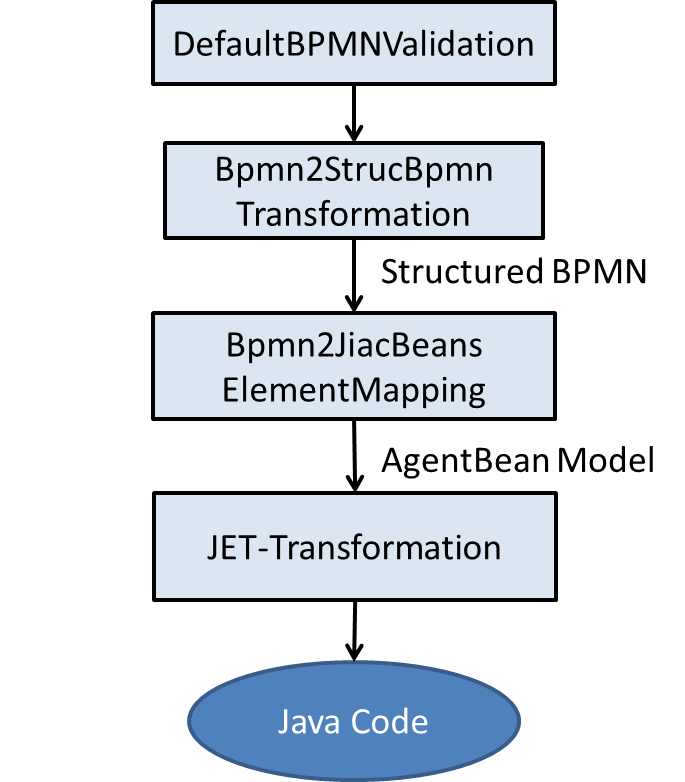
\includegraphics[width=0.4\textwidth]{images/implementation_stages.png}
	\caption{Transformation Stages}
	\label{fig:implementation_stages}
\end{figure}

Figure \ref{fig:implementation_stages} shows the structure of the transformation. Both normalization stage and structure mapping stage are implemented by the BPMN2StrucBPMN-Transformation. The clean-up stage is not included in this transformation. In the element mapping stage an intermediate Agent Bean model will be created. After the element mapping, the generated Agent Bean model will be passed into the JET-Transformation where it will be transformed into a Java file.

In the following sections we will take a closer look into the details of each transformation stage.
%===============================%
%       Validation Stage        %
%===============================%
\section{Validation}
The DefaultBPMNValidation is currently used for the validation stage. However, it might be useful to implement a new validation that checks whether the expressions given in the model are conform with the Java syntax. At the moment, some expressions are handled in the ElementMapping stage e.g. changing types to have Java conformance. Some other expressions, e.g. content of a script task, are expected to be written in Java syntax. 

%===============================%
%      Structure Mapping        %
%===============================%
\section{Normalization and Structure Mapping}
Similar to the validation stage, nothing new was implemented for the structure mapping stage. The default BPMN2StrucBPMN transformation  of the VSDT responsible for performing these two stages is being reused. 

In the normalization stage the process will be transformed into a semantically equivalent \textit{normal form}. To achieve this, the transformation uses some rules e.g. the insert gateway rule that will insert a gateway for each activity with multiple incoming or outgoing sequence flows (see example in figure \ref{fig:n+s}). The structure mapping stage is responsible for transforming the graph structured BPMN into an equivalent block structured representation. Both of the mentioned transformation stages are language independent, thus there is no need to implement a new transformation for these stages.

\begin{figure}[h]
	\centering	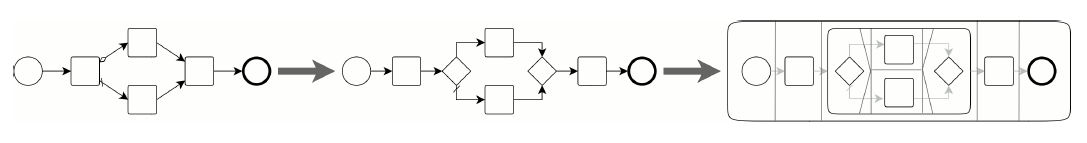
\includegraphics[width=0.9\textwidth]{images/structure_mapping.png}
	\caption{Simple Example of Normalization and Structure Mapping. \cite{TKAH08} }
	\label{fig:n+s}
\end{figure}


%===============================%
%       Element Mapping         %
%===============================%
\section{Element Mapping}
The element mapping is implemented with a visitor that will go through the elements of the process diagram with a top down traversion. In this stage, an Agent Bean Model representing a Java file holding an Agent Bean class will be generated for each pool visited in the diagram. Then the visitor will visit each element of the pool and  populate the Agent Bean model with attributes and methods according to the mapping of each visited element. 

For the implementation, the Agent Bean model was developed as an intermediate product. Let's take a closer look into the model. 
%===============================%
%       AgentBean Model         %
%===============================%
\subsection{Agent Bean Model}

An Agent Bean model has a list of attributes, methods, actions and it may also have a list of subprocesses (because a subprocess is mapped into an inner class of the generated Agent Bean).\\\\
For the content of a method, a script model was also developed. A script is basically a Java code element, which can be a single CodeElement (a single line Java code), a sequence which contains a list of scripts or even a block construct such as the while loop or a try-catch block. 

\begin{figure}[h]
	\centering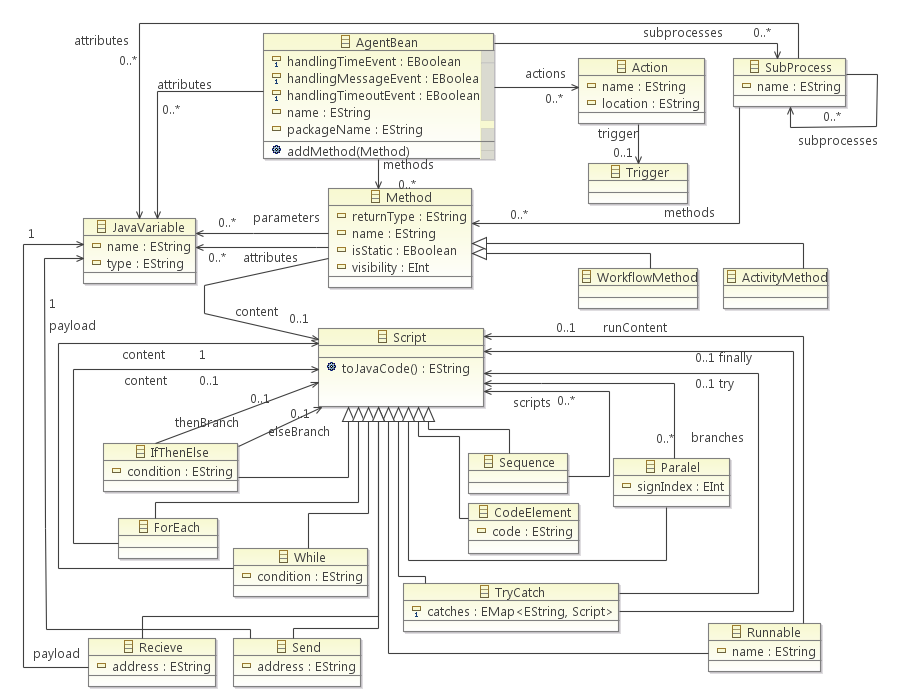
\includegraphics[width=1.0\textwidth]{images/agentBean_metamodel.png}
	\caption{Agent Bean Model}
	\label{fig:agentbean_metamodel}
\end{figure}

Each script implements the method \verb|public String toJavaCode()| which returns the java code representation of the script.
In the following listing we can see the implementation of the method in the IfThenElse class:
\begin{lstlisting}[language = Java, caption = toJavaCode() Implementation in the IfThenElse Class]
	public String toJavaCode() {
		String code = "";
		code += "if("+condition+"){\n";
		if(thenBranch!=null){
			BufferedReader reader = new BufferedReader(new StringReader(thenBranch.toJavaCode()));
			try{
				String line = reader.readLine();
				while(line!=null){
					if(!line.equals("")) code += "\t"+line+"\n";
					line = reader.readLine();
				}
			}catch(IOException e){
				code += "\t//Error occured while reading if branch\n";
			}
		}
		code+="}";
		if(elseBranch!=null){
			code+="else{\n";
			BufferedReader reader = new BufferedReader(new StringReader(elseBranch.toJavaCode()));
			try{
				String line = reader.readLine();
				while(line!=null){
					if(!line.equals("")) code += "\t"+line+"\n";
					line = reader.readLine();
				}
			}catch(IOException e){
				code += "\t//Error occured while reading else branch\n";
			}
			code+="}";
		}
		return code;
	}
\end{lstlisting}

You might notice that this method is also responsible for the text formatting because it will be used by the JET-Transformation and the result will then be written into a *.java file. For this purpose a tab is added in front of each line in the then and else branch, as you can see in line 7-11 and 21-25.\\\\
%%%%%%%%%%%%%%%%%%%%%%%%%%%
% Role of MDE             %
%%%%%%%%%%%%%%%%%%%%%%%%%%%
\textbf{The Role of MDE in the Implementation}\\\\
The benefits of Model Driven Engineering are also found during the implementation of the Agent Bean model. As we can see in figure \ref{fig:agentbean_metamodel}, the model is created graphically using eclipse's Ecore Tools - Ecore Diagram. With the help of the EMF generator each element of the model can be easily generated into Java code including a factory class that can be used to instantiate an object of each generated class. This way we only have to implement the method toJavaCode() for each newly added script, everything else are generated automatically. 


%\newpage
%%%%%%%%%%%%%%%%%%%%%%%%%%%%%%%%%%%%%%%%%%%%%%%%%%%%%%%%%%%%%%%%
%								        JET-Transformation                     %
%%%%%%%%%%%%%%%%%%%%%%%%%%%%%%%%%%%%%%%%%%%%%%%%%%%%%%%%%%%%%%%%
\section{JET-Transformation}
The JET-Transformation consists of five JET-Templates (see also figure \ref{fig:transformation_structure}): 
\begin{enumerate}
	\item agentbeantemplate.javajet
	\item subprocesstemplate.javajet
	\item timeouteventhandler.javajet
	\item timeeventhandler.javajet
	\item messageeventhandler.javajet
\end{enumerate}

\begin{figure}[h]
	\centering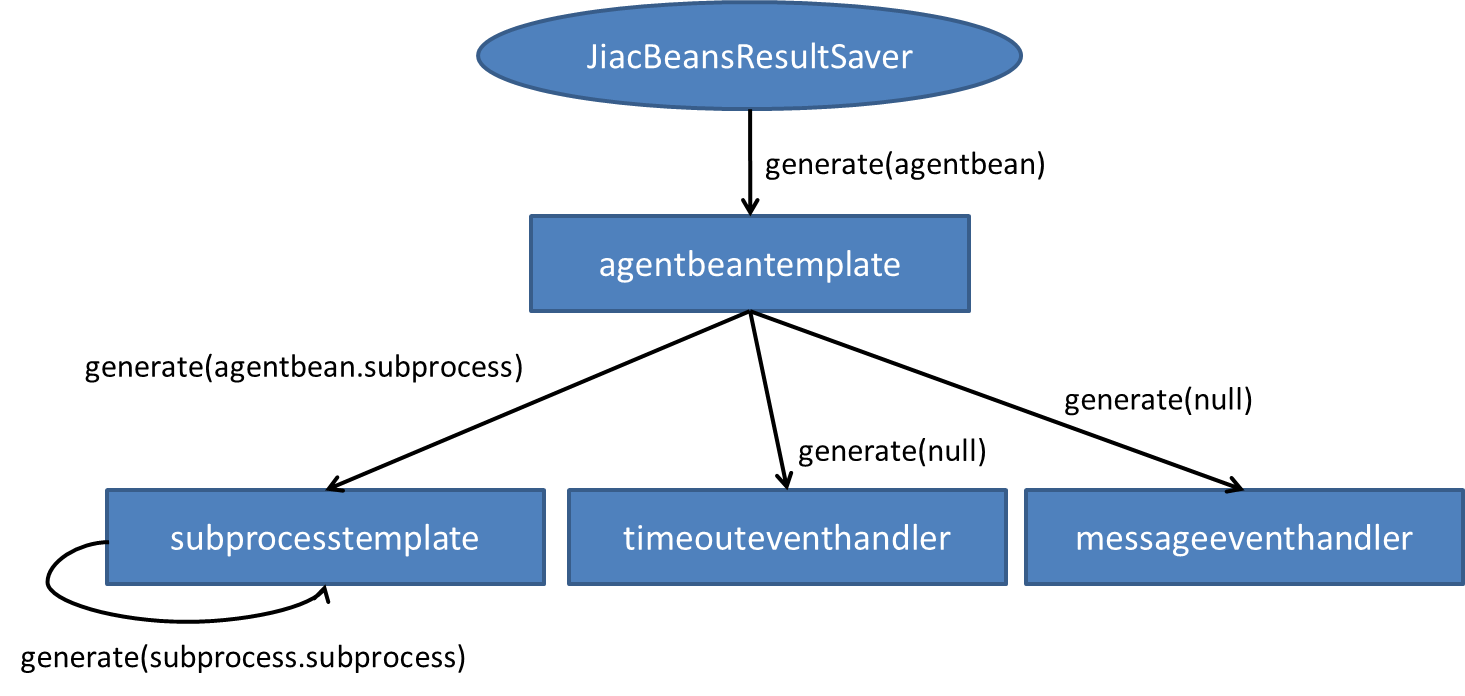
\includegraphics[width=1.0\textwidth]{images/templates_structure.png}
	\caption{JET-Transformation Structure}
	\label{fig:transformation_structure}
\end{figure}

The agentbeantemplate is the main template of the implemented JET-Transformation. An instance of its Java template class is created by the JiacBeansResultSaver and the generate method will be invoked for each Agent Bean model generated in the element mapping stage. 

The subprocesstemplate is invoked by the agentbeantemplate and recursively by the subprocesstemplate itself for each subprocess contained in their argument (an agentbean model or a subprocess model). 

The three handler templates timeouteventhandler, timeeventhandler and messageeventhandler are static templates, which means the result of the generate method does not depend on the argument object. They are responsible for generating the event handler classes TimeoutEventHandler, TimeEventHandler and MessageEventHandler. They are invoked by the agentbeantemplate if the value of the flag handlingTimeoutEvent, handlingTimeEvent or handlingMessageEvent of the Agent Bean model is true.


%%%%%%%%%%%%%%%%%%%%%%%%%%%%%%%%%%%%%%%%%%%%%%%%%%%%%%%%%%%%%%%%
%           Merging generated and manually edited code         %
%%%%%%%%%%%%%%%%%%%%%%%%%%%%%%%%%%%%%%%%%%%%%%%%%%%%%%%%%%%%%%%%
\section{Merging Generated and Manually Edited Code}
The main challenge in generating Java code is how to handle code that has been manually edited. Fortunately, the EMF comes with a solution to this problem : \textbf{JMerge}\cite{JMERGEFAQ}. With JMerge we can allow the regeneration of a model and protect manually added user code. 

We can specify some rules in an XML-file that will be loaded by JMerge.  The following listing \ref{list:mergerules} shows a very simple XML that can be used to differentiate generated elements from the the manually edited elements of a Java code. 

\begin{lstlisting}[language=xml, caption = Example JMerge Rule, label=list:mergerules]
<merge:dictionaryPattern
   name="generatedMember" 
   select="Member/getComment" 
   match="\s*@\s*(gen)erated\s*\n"/>

<merge:pull 
   targetMarkup="^gen$"
   sourceGet="Method/getBody"
   targetPut="Method/setBody"/>
\end{lstlisting}

In this case, the dictionary pattern will match code members that have the @generated annotations somewhere in their comment. The string between the parentheses in the match attribute defines the identifier which will be used in the pull element. The pull element in the example defines that the generator will replace the content of every method that has @generated in its comment.

The next thing to do is to add the comment with the @generated tags in our template for each generated elements (class, fields, methods). 
If a user edit the content of a method or the default value of a field, the @generated annotation should be deleted from the comment. Without the @generated annotation, the edited element will be let alone by JMerge and will not be lost after the regeneration of the code.  

As seen in \cite{APJMERGE}, there is a possibility to allow fine grained customization for methods and javadoc comments by using the pull elements shown in listing \ref{list:jmerge_fine}
\begin{lstlisting}[language=xml, caption=JMerge Example: fine grained customization for javadoc comments and methods, label = list:jmerge_fine]
<merge:pull 
  sourceMarkup="^gen$"
  sourceGet="Member/getComment"
  sourceTransfer="(\s*<!--\s*begin-user-doc.*?end-user-doc\s*-->\s*)\n"
  targetMarkup="^gen$"
  targetPut="Member/setComment"/>
  
<merge:pull 
   targetMarkup="^gen$"
   sourceGet="Method/getBody"
   sourceTransfer="(\s*//\s*begin-user-code.*?//\s*end-user-code\s*)\n"
   targetPut="Method/setBody"/>

\end{lstlisting}

The first pull element will allow the user to put any comments between the \verb|<!-- begin-user-doc -->| and the \verb|<!-- end-user-doc -->| tags. The second one will allow the user to customize a method by adding code between the  \verb|// begin-user-code| and \verb|// end-user-code| comments. Unfortunately, this does not seem to work if the above mentioned boundary tags and comments do not exist in the generated code. This means the position where the code may be customized should be identified in the template. For the javadoc there is no problem because the position does not matter, but for the content of a method the position cannot be predefined. Currently the javadoc comment shown in listing \ref{list:gentag} will be added to each generated variable and method.

\begin{lstlisting}[language=Java, caption = Javadoc Comment Used For JMerge, label=list:gentag]
/**
 *  <!-- begin-user-doc -->
 *  <!-- end-user-doc -->
 *	delete the generated tag after you edited this [field/method]
 *  @generated
 */
\end{lstlisting}

\subsection{Using JMerge}
In JET2, JMerge is included and can be used by adding the <java:merge/> tag somewhere in the template. However, because we are using the older version of JET we have to include JMerge in the \verb|JiacBeansResultSaver| class. At the moment, JMerge can only be used in an eclipse plugin. Listing \ref{list:using_jmerge} shows us the code needed to use JMerge.
\newpage
\begin{lstlisting}[language=java, caption=Using JMerge, label=list:using_jmerge]
ASTFacadeHelper astFacadeHelper = new ASTFacadeHelper();
JControlModel model = new JControlModel(); 
model.setLeadingTabReplacement("\t");//optional
//load the rules
model.initialize(astFacadeHelper, getClass().getResource("mergerules.xml").toString());
JMerger jMerger = new JMerger(model); 
// set the source (new generated code)
jMerger.setSourceCompilationUnit(jMerger.createCompilationUnitForContents(content));
// set the target (code from the existing file)
jMerger.setTargetCompilationUnit(jMerger.createCompilationUnitForInputStream(new FileInputStream(f))); 
// call the merge
jMerger.merge(); 
// extract the merged text
String mergedContents = jMerger.getTargetCompilationUnit().getContents();
\end{lstlisting}

\subsection{Problem with JMerge}
If the generated code contains invalid imports, e.g. if the imported target is not in the classpath, an exception will be thrown. 
To avoid this, when calling the transformation to JIAC Agent Beans, the destination folder should be a source folder in a JIAC Project\footnote{Please refer to the JIAC Manual\cite{JIACMAN10} on how to create a JIAC Project} so that all JIAC core elements needed by the Agent Bean are in the classpath. Otherwise, the code will not be merged and the existing file will be overwritten. 
%%%%%%%%%%%%%%%%%%%%%%%%%%%%%%%%%%%%%%%%%%%%%%%%%%%%%%%%%%%%%%%%
%                         Open Issues                          %
%%%%%%%%%%%%%%%%%%%%%%%%%%%%%%%%%%%%%%%%%%%%%%%%%%%%%%%%%%%%%%%%
\section{Open Issues}
\label{sec:opi}
In this chapter we presented some details of the implementation. At the moment there are still some work that have to be done regarding the implementation of the transformation such as:

\textbf{Complete the implementation of element mapping }\\
The implementation of the element mapping is not yet complete. Some concepts such as the mapping of event based gateway still have to be implemented. 

\textbf{Mixing manually edited and generated code within a method}\\
What we want is to let the user to edit only parts of the method's content by adding code within \verb|// begin-user-code| and \verb|// end-user-code|. For this purpose, either we should try to find a better mergerule or try to predefine the customizable position and use the rules shown in figure \ref{list:jmerge_fine}.

\textbf{Find a better solution for JMerge exception}\\
At the moment, the implementation will overwrite the existing code if JMerge fails to merge the code. To avoid losing manually edited code this should be changed. One solution could be by displaying a dialog where the user can choose whether to overwrite the code or to give another location for the new generated file. 
\newpage
\textbf{Identify modifiable and unmodifiable elements}\\
In the current implementation the generated members are only marked with @generated. While some elements should be modifiable by the users, some others such as the workflow method should not. We can use @unmodifiable and @modifiable to differentiate whether an element may be edited. 

\textbf{Sort generated imports}\\
Although it does not affect the validity of the generated code, the generated imports should be alphabetically sorted in order to improve the readability.




